% Created by tikzDevice version 0.10.1 on 2017-09-04 19:09:55
% !TEX encoding = UTF-8 Unicode
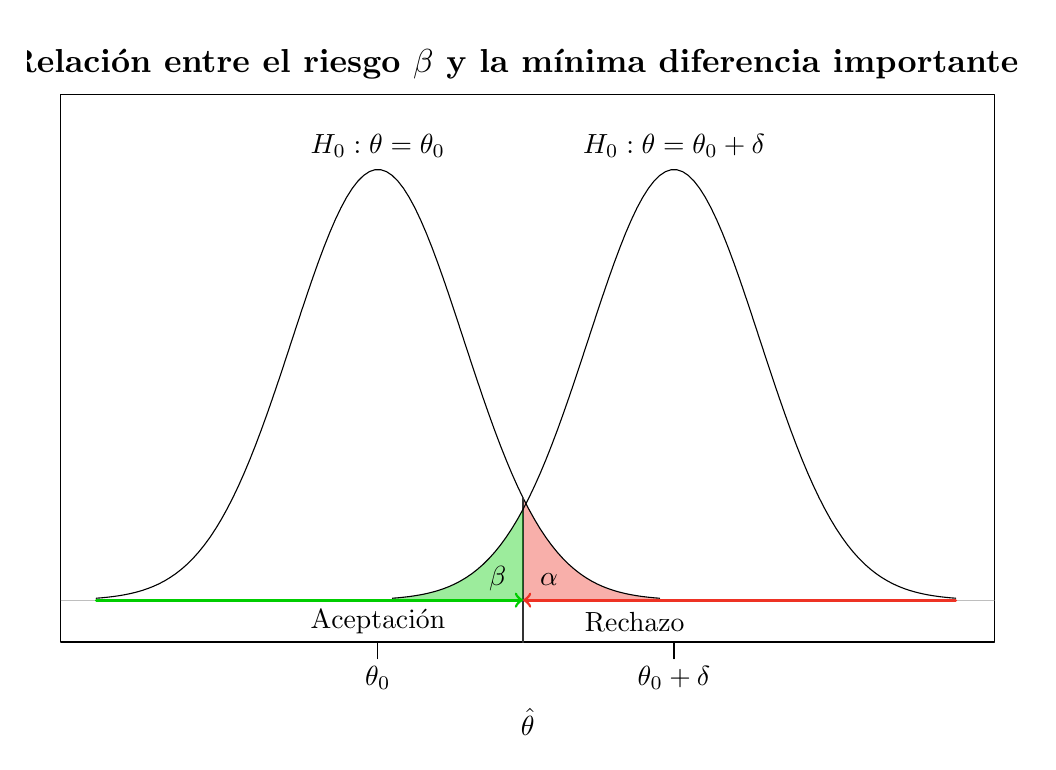
\begin{tikzpicture}[x=1pt,y=1pt]
\definecolor{fillColor}{RGB}{255,255,255}
\path[use as bounding box,fill=fillColor,fill opacity=0.00] (0,0) rectangle (361.35,258.00);
\begin{scope}
\path[clip] (  0.00,  0.00) rectangle (361.35,258.00);
\definecolor{drawColor}{RGB}{0,0,0}

\path[draw=drawColor,line width= 0.4pt,line join=round,line cap=round] ( 12.00, 36.00) --
	(349.35, 36.00) --
	(349.35,234.00) --
	( 12.00,234.00) --
	( 12.00, 36.00);
\end{scope}
\begin{scope}
\path[clip] (  0.00,  0.00) rectangle (361.35,258.00);
\definecolor{drawColor}{RGB}{0,0,0}

\node[text=drawColor,anchor=base,inner sep=0pt, outer sep=0pt, scale=  1.20] at (180.67,241.86) {\bfseries Relación entre el riesgo $\beta$ y la mínima diferencia importante $\delta$};

\node[text=drawColor,anchor=base,inner sep=0pt, outer sep=0pt, scale=  1.00] at (180.67,  2.40) {$\hat\theta$};
\end{scope}
\begin{scope}
\path[clip] ( 12.00, 36.00) rectangle (349.35,234.00);
\definecolor{drawColor}{RGB}{190,190,190}

\path[draw=drawColor,line width= 0.4pt,line join=round,line cap=round] ( 12.00, 51.14) -- (349.35, 51.14);
\definecolor{fillColor}{RGB}{238,50,36}

\path[fill=fillColor,fill opacity=0.39] (178.99, 51.14) --
	(178.99, 88.11) --
	(181.04, 84.10) --
	(183.10, 80.39) --
	(185.15, 76.98) --
	(187.21, 73.87) --
	(189.27, 71.05) --
	(191.32, 68.50) --
	(193.38, 66.21) --
	(195.43, 64.16) --
	(197.49, 62.35) --
	(199.55, 60.74) --
	(201.60, 59.33) --
	(203.66, 58.09) --
	(205.72, 57.01) --
	(207.77, 56.08) --
	(209.83, 55.28) --
	(211.88, 54.59) --
	(213.94, 54.01) --
	(216.00, 53.51) --
	(218.05, 53.09) --
	(220.11, 52.74) --
	(222.16, 52.44) --
	(224.22, 52.20) --
	(226.28, 51.99) --
	(228.33, 51.83) --
	(228.33, 51.14) --
	cycle;
\definecolor{drawColor}{RGB}{0,0,0}

\path[draw=drawColor,line width= 0.4pt,line join=round,line cap=round] ( 24.77, 51.83) --
	( 26.83, 51.99) --
	( 28.89, 52.20) --
	( 30.94, 52.44) --
	( 33.00, 52.74) --
	( 35.05, 53.09) --
	( 37.11, 53.51) --
	( 39.17, 54.01) --
	( 41.22, 54.59) --
	( 43.28, 55.28) --
	( 45.33, 56.08) --
	( 47.39, 57.01) --
	( 49.45, 58.09) --
	( 51.50, 59.33) --
	( 53.56, 60.74) --
	( 55.62, 62.35) --
	( 57.67, 64.16) --
	( 59.73, 66.21) --
	( 61.78, 68.50) --
	( 63.84, 71.05) --
	( 65.90, 73.87) --
	( 67.95, 76.98) --
	( 70.01, 80.39) --
	( 72.06, 84.10) --
	( 74.12, 88.11) --
	( 76.18, 92.43) --
	( 78.23, 97.05) --
	( 80.29,101.97) --
	( 82.35,107.16) --
	( 84.40,112.61) --
	( 86.46,118.29) --
	( 88.51,124.17) --
	( 90.57,130.22) --
	( 92.63,136.40) --
	( 94.68,142.64) --
	( 96.74,148.92) --
	( 98.79,155.16) --
	(100.85,161.31) --
	(102.91,167.31) --
	(104.96,173.10) --
	(107.02,178.61) --
	(109.08,183.79) --
	(111.13,188.56) --
	(113.19,192.88) --
	(115.24,196.69) --
	(117.30,199.94) --
	(119.36,202.60) --
	(121.41,204.62) --
	(123.47,205.98) --
	(125.52,206.67) --
	(127.58,206.67) --
	(129.64,205.98) --
	(131.69,204.62) --
	(133.75,202.60) --
	(135.81,199.94) --
	(137.86,196.69) --
	(139.92,192.88) --
	(141.97,188.56) --
	(144.03,183.79) --
	(146.09,178.61) --
	(148.14,173.10) --
	(150.20,167.31) --
	(152.26,161.31) --
	(154.31,155.16) --
	(156.37,148.92) --
	(158.42,142.64) --
	(160.48,136.40) --
	(162.54,130.22) --
	(164.59,124.17) --
	(166.65,118.29) --
	(168.70,112.61) --
	(170.76,107.16) --
	(172.82,101.97) --
	(174.87, 97.05) --
	(176.93, 92.43) --
	(178.99, 88.11) --
	(181.04, 84.10) --
	(183.10, 80.39) --
	(185.15, 76.98) --
	(187.21, 73.87) --
	(189.27, 71.05) --
	(191.32, 68.50) --
	(193.38, 66.21) --
	(195.43, 64.16) --
	(197.49, 62.35) --
	(199.55, 60.74) --
	(201.60, 59.33) --
	(203.66, 58.09) --
	(205.72, 57.01) --
	(207.77, 56.08) --
	(209.83, 55.28) --
	(211.88, 54.59) --
	(213.94, 54.01) --
	(216.00, 53.51) --
	(218.05, 53.09) --
	(220.11, 52.74) --
	(222.16, 52.44) --
	(224.22, 52.20) --
	(226.28, 51.99) --
	(228.33, 51.83);

\node[text=drawColor,anchor=base,inner sep=0pt, outer sep=0pt, scale=  1.00] at (126.55,212.47) {$H_0: \theta = \theta_0$};
\definecolor{drawColor}{gray}{0.20}

\path[draw=drawColor,line width= 0.4pt,line join=round,line cap=round] (178.99, 12.13) -- (178.99, 88.11);
\definecolor{drawColor}{RGB}{0,0,0}

\node[text=drawColor,anchor=base,inner sep=0pt, outer sep=0pt, scale=  1.00] at (188.41, 56.44) {$\alpha$};
\end{scope}
\begin{scope}
\path[clip] (  0.00,  0.00) rectangle (361.35,258.00);
\definecolor{drawColor}{RGB}{0,0,0}

\path[draw=drawColor,line width= 0.4pt,line join=round,line cap=round] (126.55, 36.00) -- (126.55, 36.00);

\path[draw=drawColor,line width= 0.4pt,line join=round,line cap=round] (126.55, 36.00) -- (126.55, 30.00);

\node[text=drawColor,anchor=base,inner sep=0pt, outer sep=0pt, scale=  1.00] at (126.55, 20.40) {$\theta_0$};
\end{scope}
\begin{scope}
\path[clip] ( 12.00, 36.00) rectangle (349.35,234.00);
\definecolor{drawColor}{RGB}{0,205,0}

\path[->, draw=drawColor,line width= 1.0pt,line join=round,line cap=round] ( 24.77, 51.14) -- (178.99, 51.14);
\definecolor{drawColor}{RGB}{238,50,36}

\path[->, draw=drawColor,line width= 1.0pt,line join=round,line cap=round] (335.34, 51.14) -- (178.99, 51.14);
\definecolor{drawColor}{RGB}{0,0,0}

\node[text=drawColor,anchor=base,inner sep=0pt, outer sep=0pt, scale=  1.00] at (126.55, 40.86) {Aceptación};

\node[text=drawColor,anchor=base,inner sep=0pt, outer sep=0pt, scale=  1.00] at (219.33, 39.89) {Rechazo};
\definecolor{fillColor}{RGB}{0,205,0}

\path[fill=fillColor,fill opacity=0.39] (131.78, 51.14) --
	(131.78, 51.83) --
	(133.84, 51.99) --
	(135.89, 52.20) --
	(137.95, 52.44) --
	(140.00, 52.74) --
	(142.06, 53.09) --
	(144.12, 53.51) --
	(146.17, 54.01) --
	(148.23, 54.59) --
	(150.29, 55.28) --
	(152.34, 56.08) --
	(154.40, 57.01) --
	(156.45, 58.09) --
	(158.51, 59.33) --
	(160.57, 60.74) --
	(162.62, 62.35) --
	(164.68, 64.16) --
	(166.73, 66.21) --
	(168.79, 68.50) --
	(170.85, 71.05) --
	(172.90, 73.87) --
	(174.96, 76.98) --
	(177.02, 80.39) --
	(179.07, 84.10) --
	(179.07, 51.14) --
	cycle;

\path[draw=drawColor,line width= 0.4pt,line join=round,line cap=round] (131.78, 51.83) --
	(133.84, 51.99) --
	(135.89, 52.20) --
	(137.95, 52.44) --
	(140.00, 52.74) --
	(142.06, 53.09) --
	(144.12, 53.51) --
	(146.17, 54.01) --
	(148.23, 54.59) --
	(150.29, 55.28) --
	(152.34, 56.08) --
	(154.40, 57.01) --
	(156.45, 58.09) --
	(158.51, 59.33) --
	(160.57, 60.74) --
	(162.62, 62.35) --
	(164.68, 64.16) --
	(166.73, 66.21) --
	(168.79, 68.50) --
	(170.85, 71.05) --
	(172.90, 73.87) --
	(174.96, 76.98) --
	(177.02, 80.39) --
	(179.07, 84.10) --
	(181.13, 88.11) --
	(183.18, 92.43) --
	(185.24, 97.05) --
	(187.30,101.97) --
	(189.35,107.16) --
	(191.41,112.61) --
	(193.46,118.29) --
	(195.52,124.17) --
	(197.58,130.22) --
	(199.63,136.40) --
	(201.69,142.64) --
	(203.75,148.92) --
	(205.80,155.16) --
	(207.86,161.31) --
	(209.91,167.31) --
	(211.97,173.10) --
	(214.03,178.61) --
	(216.08,183.79) --
	(218.14,188.56) --
	(220.19,192.88) --
	(222.25,196.69) --
	(224.31,199.94) --
	(226.36,202.60) --
	(228.42,204.62) --
	(230.48,205.98) --
	(232.53,206.67) --
	(234.59,206.67) --
	(236.64,205.98) --
	(238.70,204.62) --
	(240.76,202.60) --
	(242.81,199.94) --
	(244.87,196.69) --
	(246.92,192.88) --
	(248.98,188.56) --
	(251.04,183.79) --
	(253.09,178.61) --
	(255.15,173.10) --
	(257.21,167.31) --
	(259.26,161.31) --
	(261.32,155.16) --
	(263.37,148.92) --
	(265.43,142.64) --
	(267.49,136.40) --
	(269.54,130.22) --
	(271.60,124.17) --
	(273.66,118.29) --
	(275.71,112.61) --
	(277.77,107.16) --
	(279.82,101.97) --
	(281.88, 97.05) --
	(283.94, 92.43) --
	(285.99, 88.11) --
	(288.05, 84.10) --
	(290.10, 80.39) --
	(292.16, 76.98) --
	(294.22, 73.87) --
	(296.27, 71.05) --
	(298.33, 68.50) --
	(300.39, 66.21) --
	(302.44, 64.16) --
	(304.50, 62.35) --
	(306.55, 60.74) --
	(308.61, 59.33) --
	(310.67, 58.09) --
	(312.72, 57.01) --
	(314.78, 56.08) --
	(316.83, 55.28) --
	(318.89, 54.59) --
	(320.95, 54.01) --
	(323.00, 53.51) --
	(325.06, 53.09) --
	(327.12, 52.74) --
	(329.17, 52.44) --
	(331.23, 52.20) --
	(333.28, 51.99) --
	(335.34, 51.83);
\end{scope}
\begin{scope}
\path[clip] (  0.00,  0.00) rectangle (361.35,258.00);
\definecolor{drawColor}{RGB}{0,0,0}

\path[draw=drawColor,line width= 0.4pt,line join=round,line cap=round] (233.56, 36.00) -- (233.56, 36.00);

\path[draw=drawColor,line width= 0.4pt,line join=round,line cap=round] (233.56, 36.00) -- (233.56, 30.00);

\node[text=drawColor,anchor=base,inner sep=0pt, outer sep=0pt, scale=  1.00] at (233.56, 20.40) {$\theta_0+\delta$};
\end{scope}
\begin{scope}
\path[clip] ( 12.00, 36.00) rectangle (349.35,234.00);
\definecolor{drawColor}{RGB}{0,0,0}

\node[text=drawColor,anchor=base,inner sep=0pt, outer sep=0pt, scale=  1.00] at (233.56,212.47) {$H_0: \theta = \theta_0 + \delta$};

\node[text=drawColor,anchor=base,inner sep=0pt, outer sep=0pt, scale=  1.00] at (169.85, 56.44) {$\beta$};
\end{scope}
\end{tikzpicture}
